\documentclass[10pt,a4paper]{article}
\usepackage[utf8]{inputenc}
\usepackage[T1]{fontenc}
\usepackage[spanish]{babel}
\usepackage{amsmath}
\usepackage{amsfonts}
\usepackage{amssymb}
\usepackage{graphicx}
\begin{document}
	\section{Amplitud Modulada}
	Es el proceso de cambiar la amplitud de una señal portadora de frecuencia relativamente alta, en proporción con el valor instantáneo de la señal modulante o moduladora. La modulación de amplitud es una forma de modulación relativamente poco costosa y de baja calidad, que se usa para emisiones comerciales de señales de audio y de video.
	\\
	La portadora se representa con la expresion:
	\begin{align}
	V_c\sin(2\pi f_c t)
	\end{align}
	La señal moduladora:
	\begin{align}
		V_m\sin (2\pi f_m t)
	\end{align}
	La onda modulada
	\begin{align}
		V_{am}
	\end{align}
	\begin{center}
		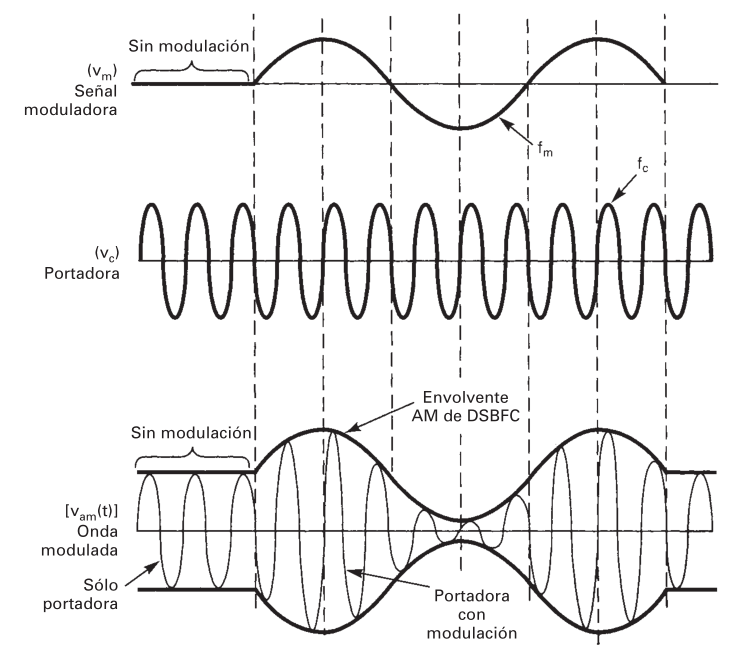
\includegraphics[scale=0.5]{screenshot001}
	\end{center}
	\subsection{Coeficiente de modulación}
	Un termino que describe la cantidad de cambio de amplitud que hay en una forma de onda de AM es el coeficiente de modulación expresado como porcentaje. El porcentaje de modulación indica el cambio porcentual de amplitud de la onda de salida cuando sobre la portadora actua una señal moduladora. Coeficiente de modulación es:
	\begin{align}
		m=\frac{E_m}{E_c}
	\end{align}
	Donde m es el coeficiente de modulación, $E_m$ cambio máximo de amplitud de la forma de onda de voltaje de salida (volts), $E_c$ amplitud máxima del voltaje de la portadora no modulada (volts).
	\subsection{Distribución de voltaje de AM}
	Una portadora no modulada se puede describir matematicamente com sigue:
	\begin{align}
		v_c(t)=E_c \sin(2\pi f_c t)
	\end{align}
	La amplitud instantánea de la onda modulada se puede expresar como sigue:
	\begin{align}
		v_am(t)=[E_c+E_m \sin (2\pi f_m t)][\sin(2\pi f_c t)]
	\end{align}
	sustituyendo $E_m$ por $mE_c$ y sacando factor común $E_c$:
		\begin{align}
		v_{am}(t)=[1+m\sin(2\pi f_m t)][E_c\sin(2\pi f_c t)]
	\end{align}	
	Desarrollando la ecuación anterior:
	\begin{align}
		v_{am}(t)=E_c\sin(2\pi f_c t)-\frac{mE_c}{2}\cos[2\pi(f_c+f_m)t]+\frac{mE_c}{2}\cos[2\pi(f_c-f_m)t]
	\end{align}
	\begin{center}
		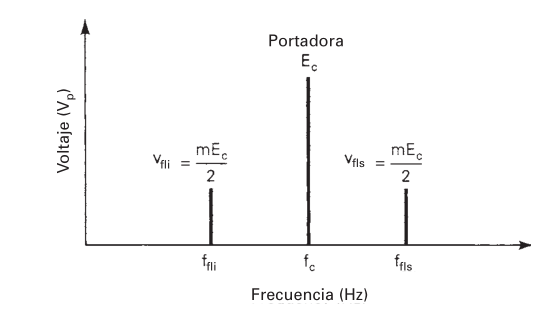
\includegraphics[scale=0.5]{screenshot002}
	\end{center}
	\subsection{Distribución de potencia en AM}
	El promedio de la potencia disipada en una carga, por una portadora no modulada es igual al cuadrado del voltaje rms de la portadora, dividido entre la resistencia de carga. Esto se expresa:
	\begin{align}
		P_c=\frac{(\sqrt{2}E_c)^2}{R}=\frac{(E_c)^2}{2R}
	\end{align}
	Siendo $P_c$ potencia de la portadora (watts), $E_c$ voltaje maximo de la portadora (volts).
	
\end{document}